\documentclass[main.tex]{subfiles}

\begin{document}

\section{Appendix A - User Manual}
\label{user_manual}

\subsection{Launching Thalia}
Since Thalia is a web application, it can be accessed from your web browser at the address: \urllink{http://thaliabacktest.xyz/}{http://thaliabacktest.xyz/}.

\begin{figure}[H]
   \centering
   
\includegraphics[scale=0.8]{08Appendices/081User/081Pictures/thalia_domain.png}
   \caption{Thalia Web}
   \label{thalia_web}
\end{figure}

\subsection{Browsing Thalia}

The application can be navigated using the navigation bar, visible on \figurename{\ref{thalia_navbar}}.

\begin{figure}[H]
   \centering
   
\includegraphics[width=\textwidth]{08Appendices/081User/081Pictures/navbar.png}
   \caption{Thalia Navigation Bar}
   \label{thalia_navbar}
\end{figure}

In case Thalia is launched on a different device, such as mobile, or in a smaller window on your desktop, the layout will change to fit the screen. In this case, the navigation bar becomes a so-called ``hamburger button`` and dropdown as can be seen on \figurename{\ref{thalia_navbar_hamburger}}.

\begin{figure}[H]
   \centering
   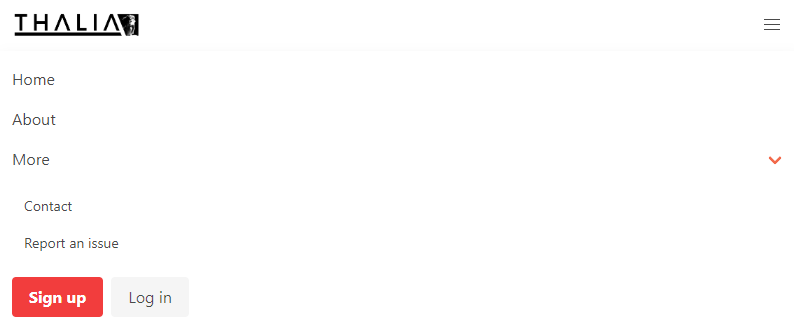
\includegraphics[width=\textwidth]{08Appendices/081User/081Pictures/navbar_hamburger.png}
   \caption{Thalia Navigation Bar - Hamburger}
   \label{thalia_navbar_hamburger}
\end{figure}

For the rest of this manual, we shall assume that the application is being accessed from a desktop computer, although the layout is much the same and equally intuitive on both desktop and mobile displays.

\subsubsection{Homepage}
By default, the user is directed to the homepage, although some of the other pages can also be accessed by providing the correct URL. The following image depicts the homepage:

\figurename{\ref{thalia_home}}.
\begin{figure}[H]
   \centering
   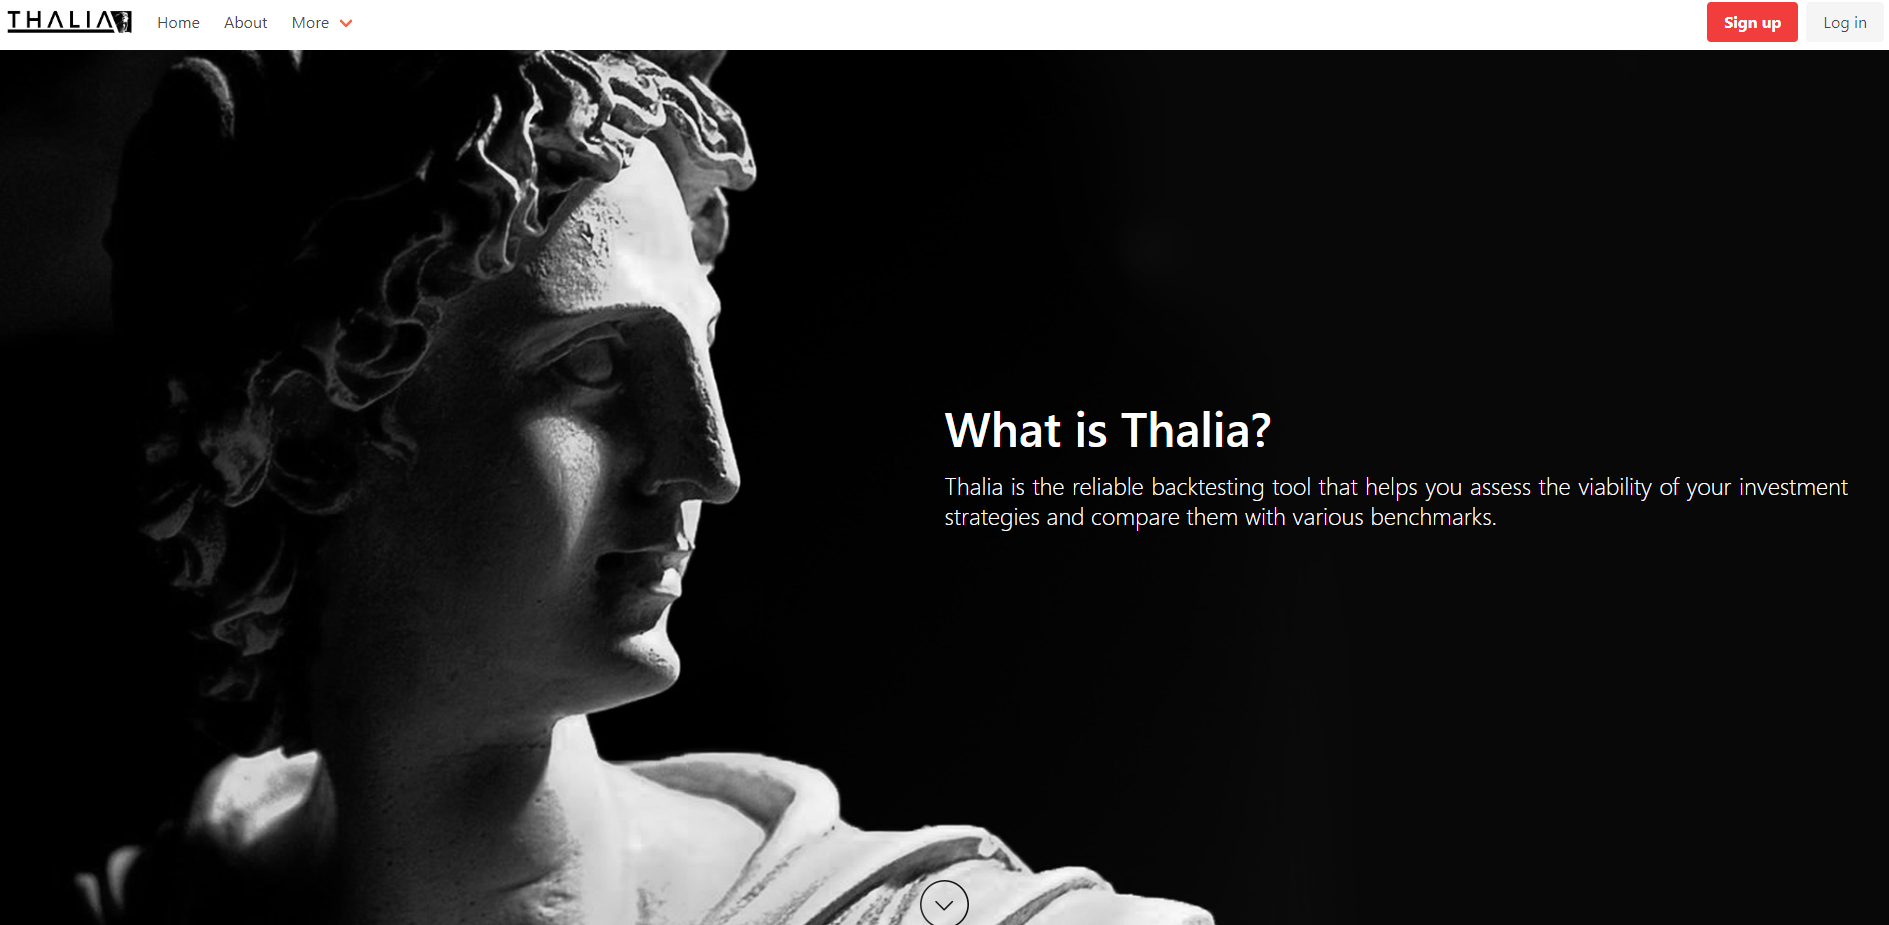
\includegraphics[width=\textwidth]{08Appendices/081User/081Pictures/homepage.png}
   \caption{Thalia Homepage (source: http://thaliabacktest.xyz/)}
   \label{thalia_home}
\end{figure}

The purpose of the homepage is to provide our application with a cover. When users arrive at the homepage, they are greeted by a short description of what our software can do.

As we do not wish to have users jumping blindly into portfolio analysis, we provide them with some basic information on the backtesting process. A link at the end of the description leads to the `About` page, where users can read up on the topic in greater detail.

Scrolling further down, the user may encounter a short register form, or if the user is logged in, an embedding of our Twitter timeline. At the bottom of most pages you can find a footer with links to our social media and a short legal disclaimer to better define the service we are offering.

\begin{figure}[H]
   \centering
   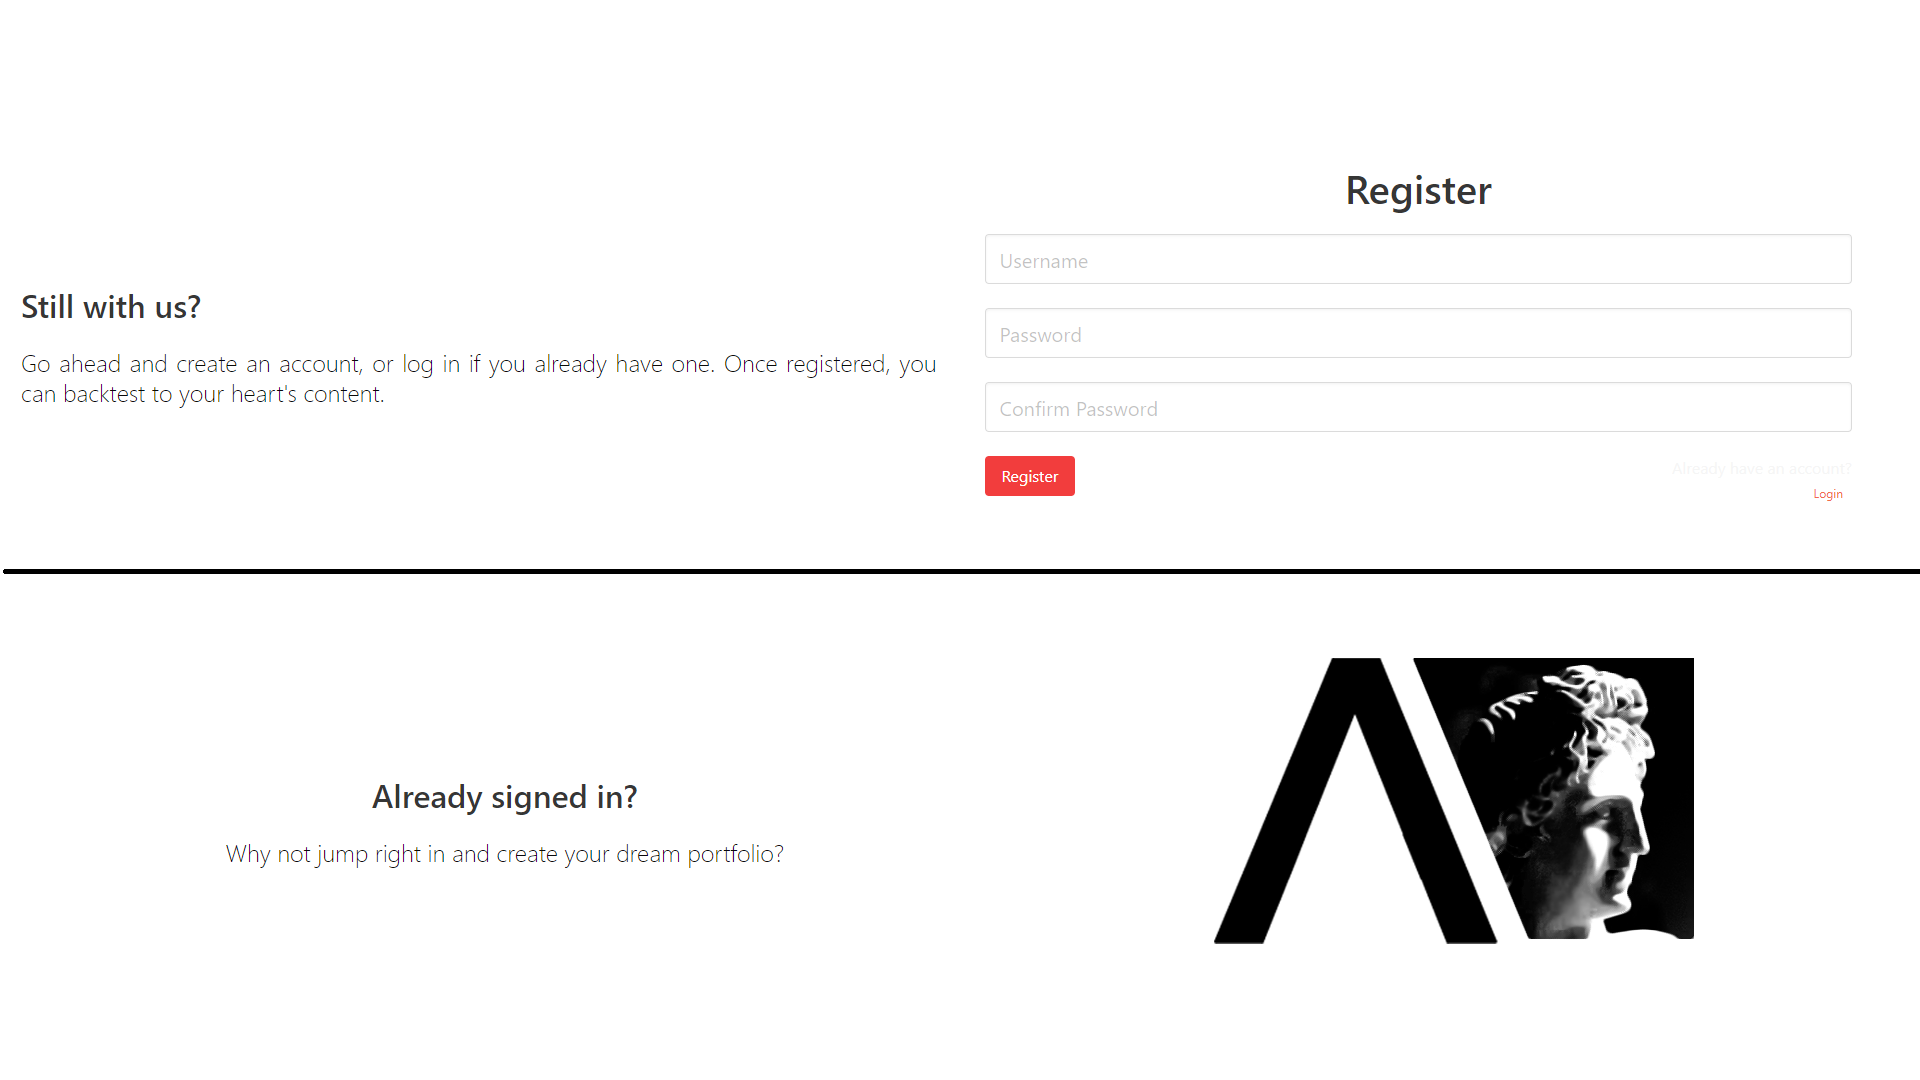
\includegraphics[width=\textwidth]{08Appendices/081User/081Pictures/homepage_bottom.png}
   \caption{Top: User not logged in; Bottom: User recognised}
   \label{thalia_home_bottom}
\end{figure}

\subsubsection{About Page}
The about page of our application provides a more detailed description of the problem domain and is available at \urllink{http://thaliabacktest.xyz/about/}{http://thaliabacktest.xyz/about/}.

The user can access this page by either directly typing the URL into the address bar, by clicking on the learn more button on the homepage, or by navigating to it using the navigation bar.

The about page looks as follows:

\begin{figure}[H]
   \centering
   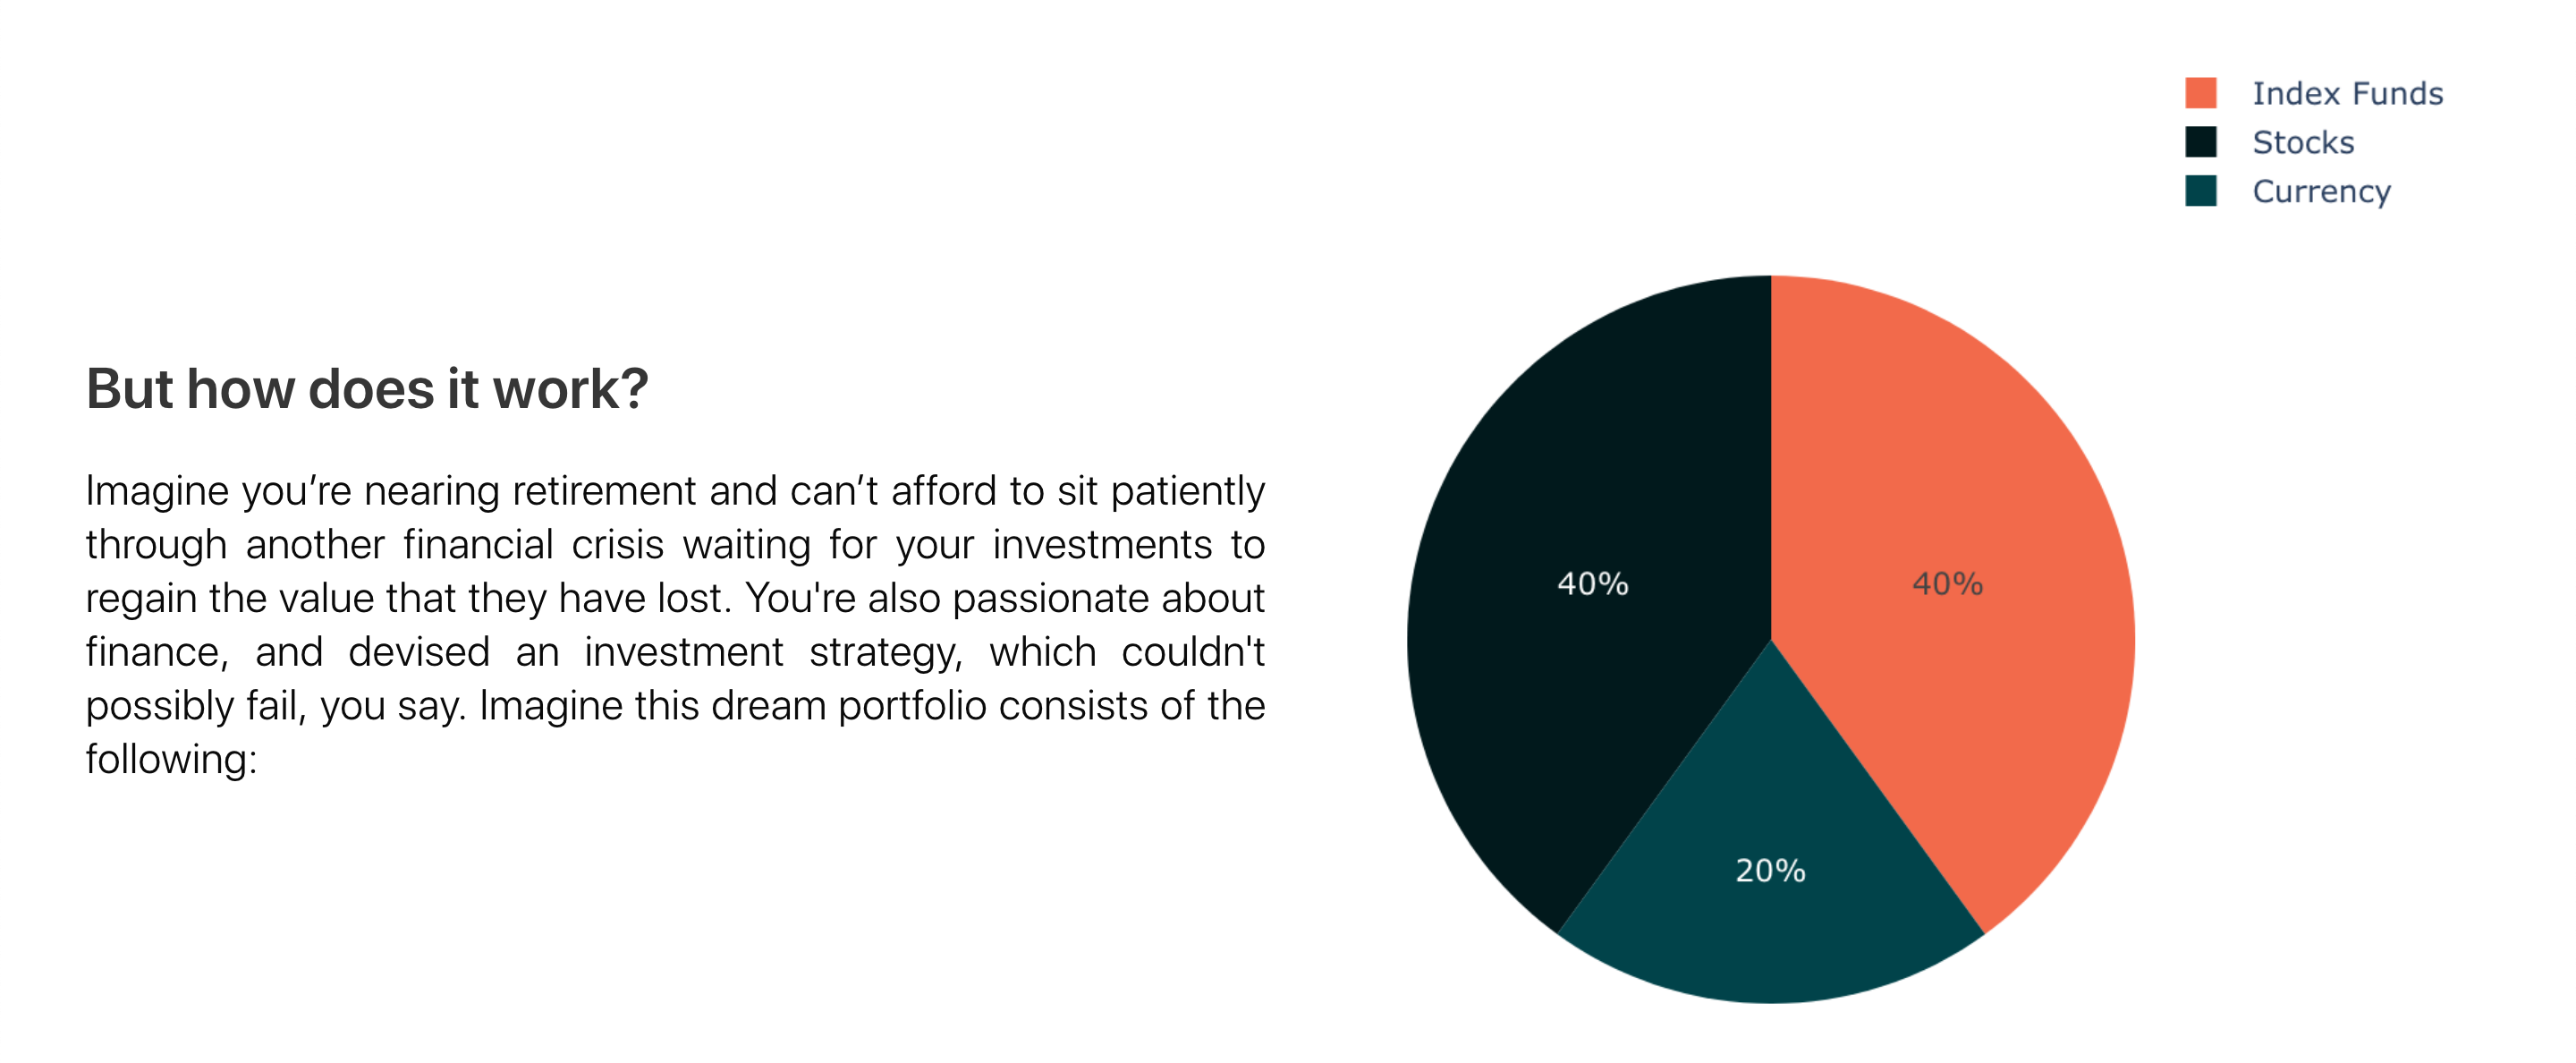
\includegraphics[width=\textwidth,keepaspectratio]{08Appendices/081User/081Pictures/about_1.png}
   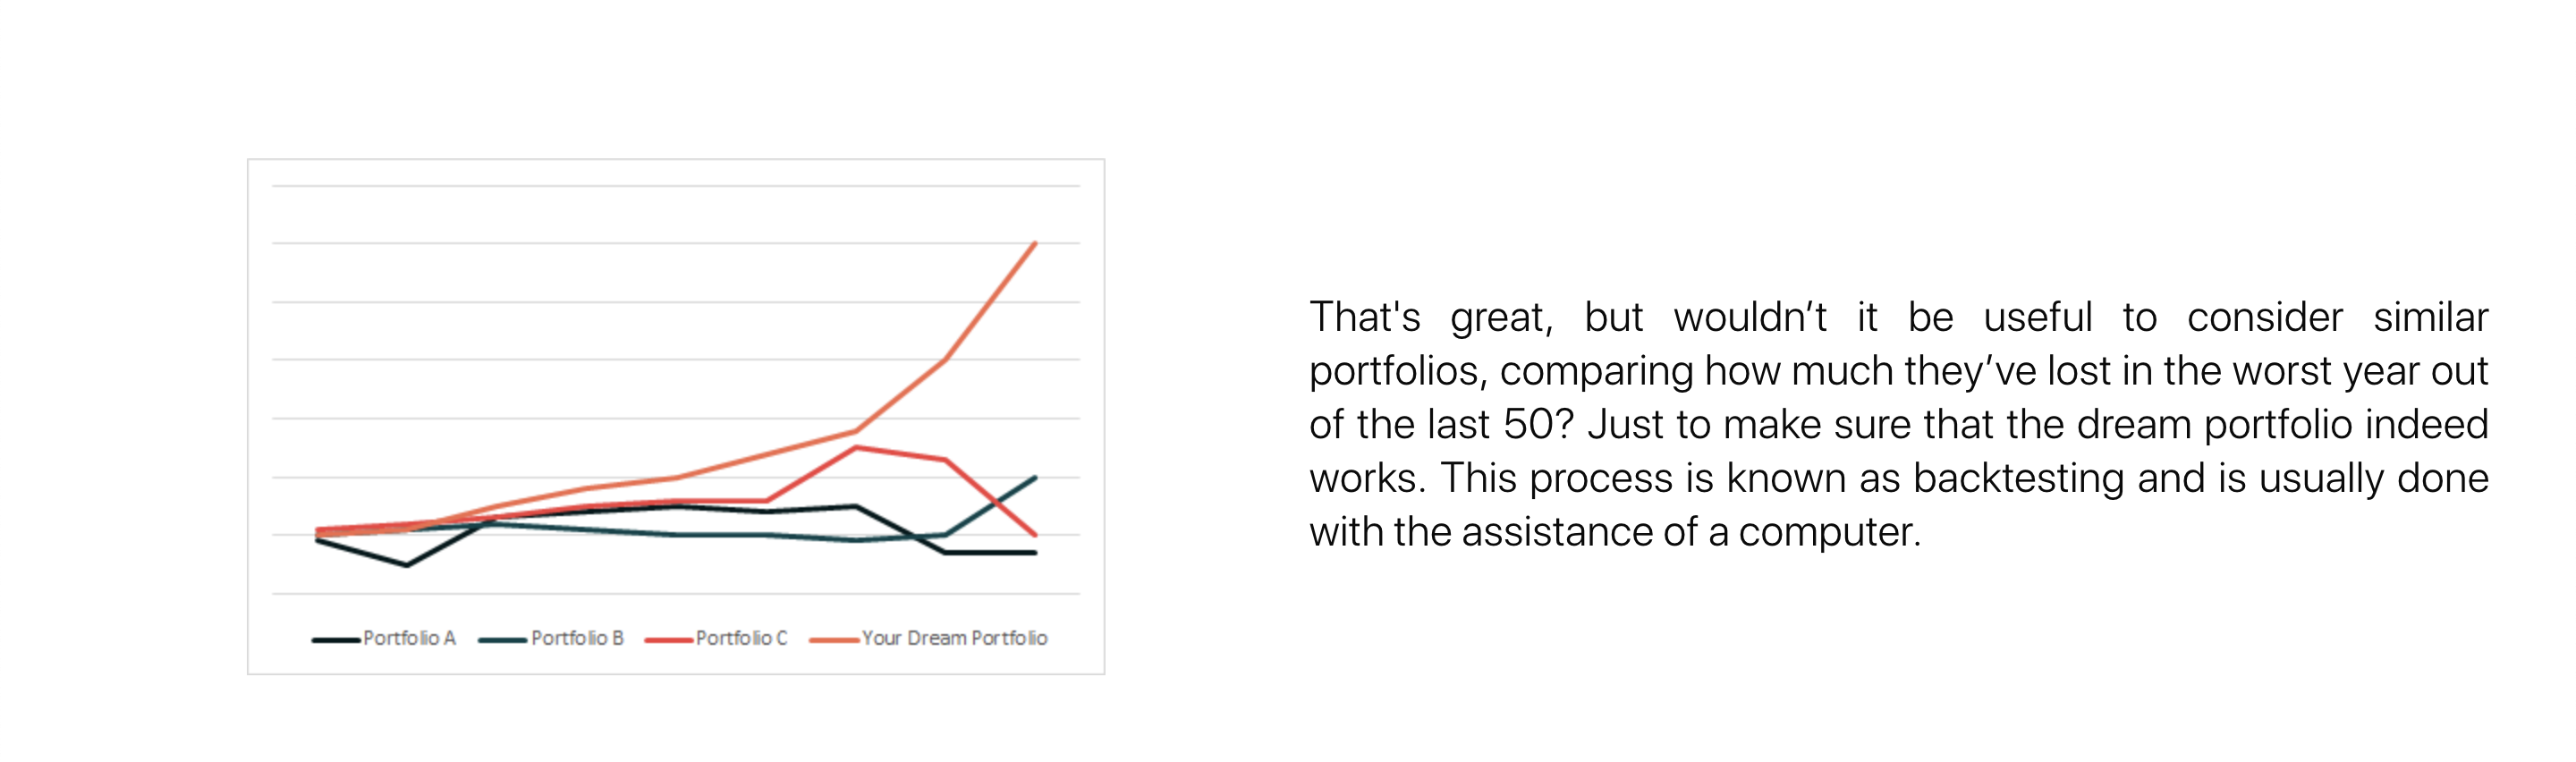
\includegraphics[width=\textwidth,keepaspectratio]{08Appendices/081User/081Pictures/about_2.png}
   
\includegraphics[width=\textwidth,keepaspectratio]{08Appendices/081User/081Pictures/about_3.png}
   \caption{Thalia About Page (source: http://thaliabacktest.xyz/about/)}
   \label{thalia_about}
\end{figure}

\subsubsection{Log In and Sign Up Pages}
IF the user is not yet logged in, links to the `Log In` and `Sign Up` pages are visible on the right hand side of the navigation bar as seen on \figurename{\ref{thalia_navbar}} or \figurename{\ref{thalia_navbar_hamburger}}. In addition, they are directly available at \urllink{http://thaliabacktest.xyz/login/}{http://thaliabacktest.xyz/login/} and \urllink{http://thaliabacktest.xyz/register/}{http://thaliabacktest.xyz/register/}.

Both of these forms follow a standard layout, with the login requiring:

\begin{itemize}
    \item Username
    \item Password
    \item Remember me (optional)
\end{itemize}

For the sign up form, the fields are:

\begin{itemize}
    \item Username
    \item Password (minimum eight characters, at least one letter, one number and one special character)
    \item Confirm Password
\end{itemize}

By convention, the registration fails when the user enters different values to the Password and Confirm Password fields. In this case, the user is prompted to try again.

\begin{figure}[H]
   \centering
   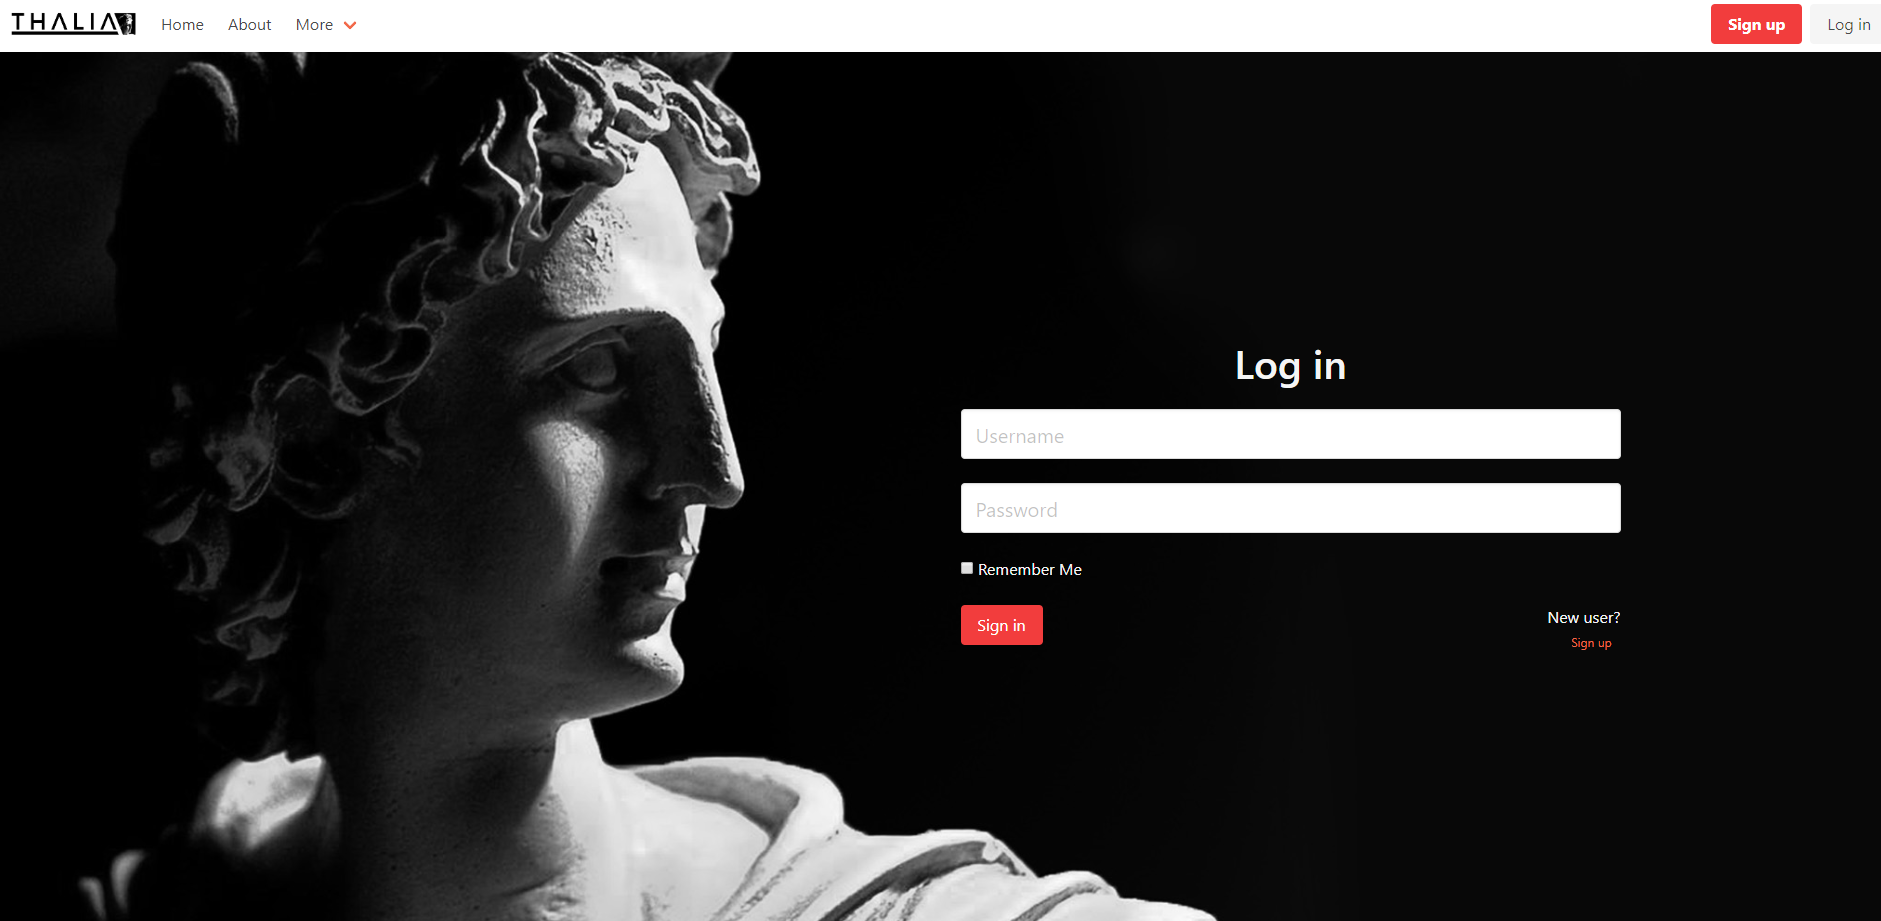
\includegraphics[width=\textwidth]{08Appendices/081User/081Pictures/login.png}
   \caption{Thalia Log In Page (source: http://thaliabacktest.xyz/login/)}
   \label{thalia_login}
\end{figure}

If the user is already logged in and attempts to access these pages, they will be redirected to the homepage. In addition, the navigation bar changes, allowing one to log out as visible on \figurename{\ref{thalia_issues}}.

After clicking the log out button, the user will find themselves back on the homepage.

\subsubsection{Contact Us Page}

The `Contact Us` page is available at \urllink{http://thaliabacktest.xyz/contact/}{http://thaliabacktest.xyz/contact/} or by opening the dropdown menu on the navigation bar and clicking the link. This short form allows users to provide feedback, report issues or request new features.

\begin{figure}[H]
   \centering
   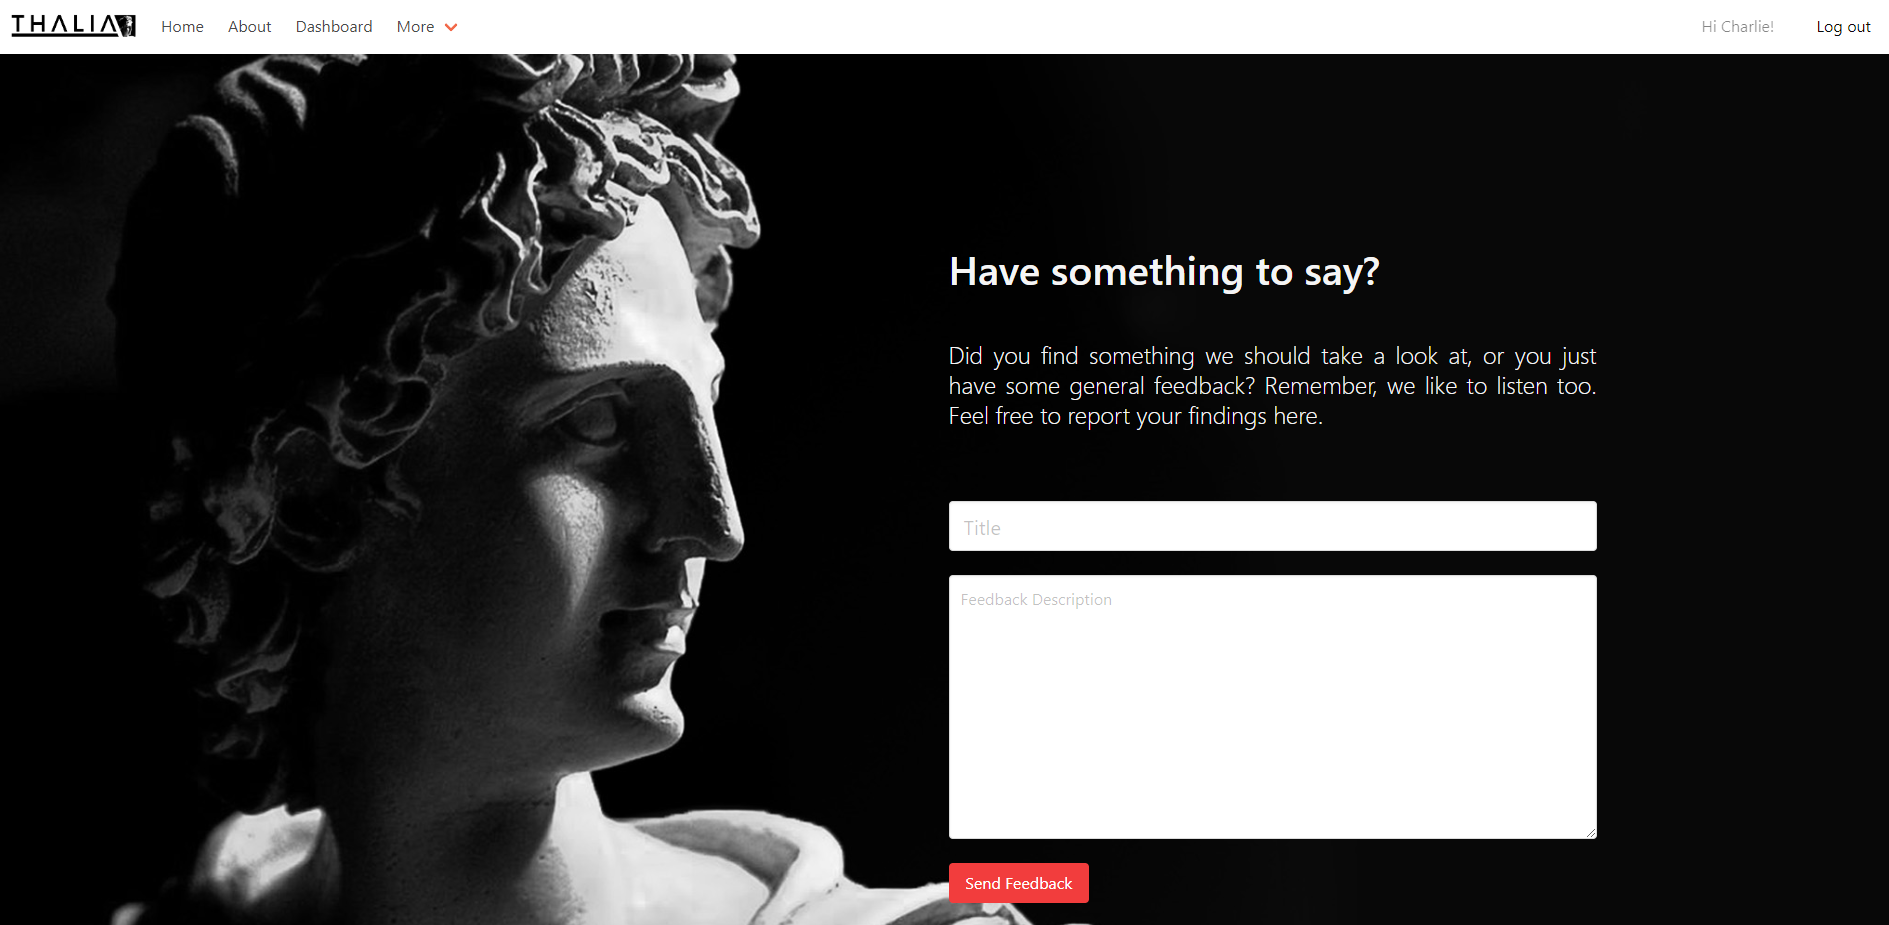
\includegraphics[width=\textwidth]{08Appendices/081User/081Pictures/issues.png}
   \caption{Thalia Report Issues Page (source: http://thaliabacktest.xyz/contact/)}
   \label{thalia_issues}
\end{figure}

\subsubsection{About Us Page}
We take great pride in our project and thus wanted to sign our work following the advice in \cite{pragmaticprog}. This simple page is dedicated to the team behind Thalia.

\subsubsection{My Portfolios Page}

The `My Portfolios` Page is only accessible to authenticated users. Here, the user may view their saved portfolios and their asset allocations. If you are running Thalia for the first time, this page will be empty, encouraging you to go create and save a portfolio.
To create a portfolio, simply head to the dashboard and allocate your assets following the instructions in \ref{create_portfolio}. Before submitting your investment strategy, make sure to save it for later. You can achieve this by clicking on the default portfolio name and changing it to something more fitting. Then, click the `Save Portfolio` button. When you next visit the `My Portfolios` Page, you can see the portfolio and its associated asset weights. Clicking on the box will take you back to the dashboard. The corresponding allocations will already be loaded to the table. Alternatively, you can select any of your previously saved portfolios directly from the dashboard by using the dropdown menu and selecting your chosen portfolio.

The following image shows the aforementioned page with some example portfolios saved.
\begin{figure}[H]
   \centering
   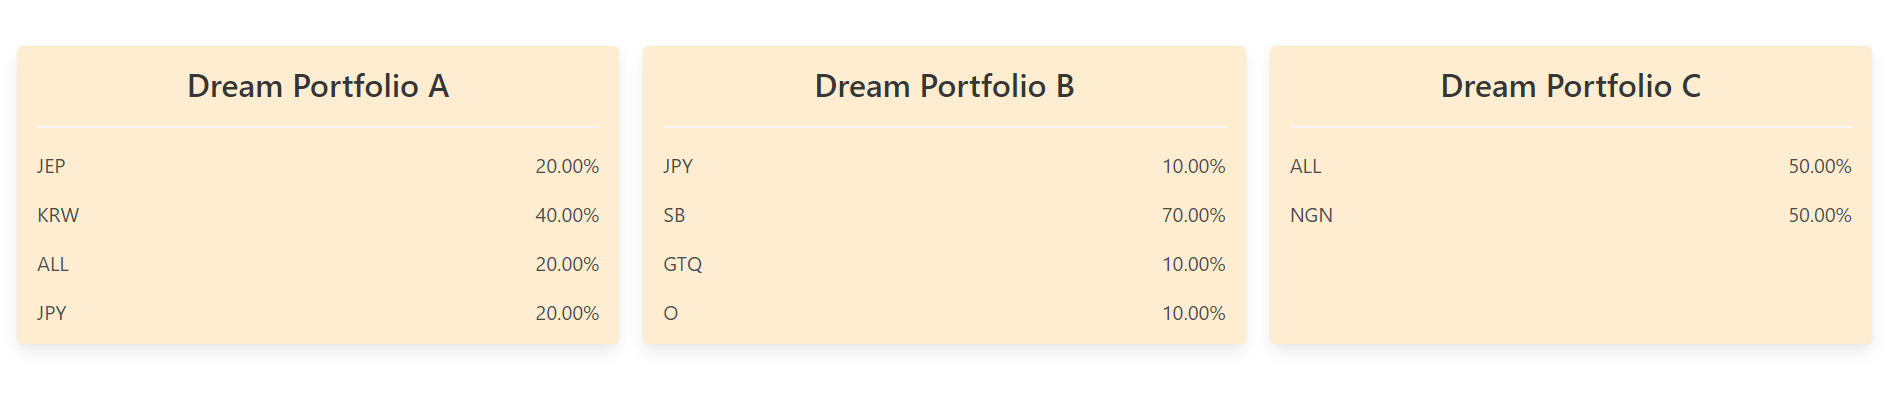
\includegraphics[width=\textwidth]{08Appendices/081User/081Pictures/my_portfolios.png}
   \caption{My Portfolios - Example (source: http://thaliabacktest.xyz/gallery/)}
\end{figure}

\subsection{Running a Backtest}

To run a backtest, the user must be authenticated. After a successful registration and/or login process, the user can head to the Dashboard and begin backtesting.

\subsubsection{Dashboard}

The Dashboard, witch is at the heart of our application, is available for registered users at \urllink{http://thaliabacktest.xyz/dashboard/}{http://thaliabacktest.xyz/dashboard/} or via the link on the navigation bar.

This web page is divided into the following tabs:

\begin{itemize}
    \item Ticker Selector
    \item Summary
    \item Metrics
    \item Returns 
    \item Drawdowns
    \item Assets
    \item Overfitting
\end{itemize}

At first, only the Ticker Selector Page is accessible to the user. 

This is because the remaining tabs are used to display the results of backtesting one or multiple portfolios and consequently do not initially contain any data.

\begin{figure}[H]
   \centering
   
\includegraphics[width=\textwidth]{08Appendices/081User/081Pictures/disabled_tabs.png}
   \caption{Thalia Dashboard - Disabled Tabs}
   \label{thalia_disabled_tabs}
\end{figure}

Let us now consider each tab individually. 

\subsubsection{Ticker Selector}

\label{create_portfolio}

Here, the user is required to input their backtesting strategy. As Thalia supports testing multiple portfolios at once (currently up to 5), there are two types of input field. Those that are portfolio specific and those that are not. The latter consists of:

\begin{itemize}
    \item Start Date: The day the investment is made.
    \item End Date: The last day of the investment, which defaults to the present date.
    \item Initial Amount: Initial balance. The default currency is dollars, as is convention for financial applications.
\end{itemize}

The first two of these are standard date-selectors, but also allow for typing the date directly. Next, the user enters the data specific to the current strategy.

\begin{itemize}
    \item Portfolio Name: Defaults to Portfolio 1, Portfolio 2, etc. 
    \item Contribution Amount: The amount that should be added to the total investments on a regular basis (e.g. after receiving a monthly paycheck).
    \item Contribution Frequency: Specify how regularly these contributions should occur.
    \item Rebalancing Frequency: Specify how often rebalancing (reestablishing the initial weights of the portfolio by buying and selling assets) should happen. 
    \item Asset Allocations: Discussed below.
\end{itemize}

The last one is the most crucial information in a strategy. First, the user selects the desired asset from the dropdown menu. The menu item also allows for input to be typed in order to find an asset faster. The selected item is then added into the table below.

\begin{figure}[H]
   \centering
   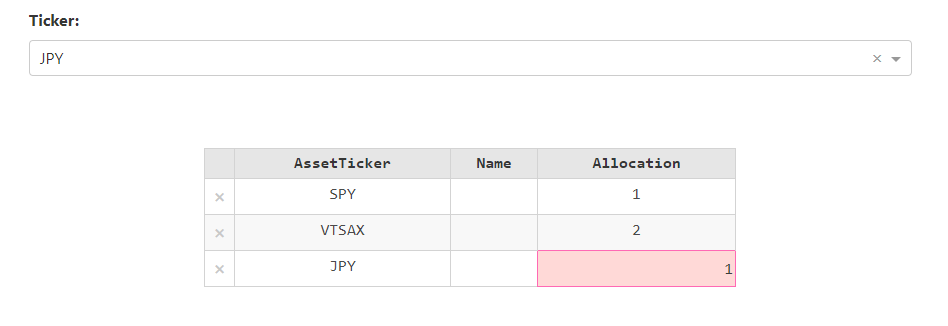
\includegraphics[width=\textwidth]{08Appendices/081User/081Pictures/table.png}
   \caption{Thalia Dashboard - Asset Table (source: http://thaliabacktest.xyz/dashboard/)}
   \label{thalia_table}
\end{figure}


The user then specifies the weight of the asset in their portfolio. This must be a numeric value, representing the \textit{relative} weight of the asset. For example, given asset A with relative weight 1, and asset B with relative weight 2, then 33\% of the investment is allocated to asset A and 66\% to asset B.

If the user is content with the portfolio, they can either add another strategy via the ``Add Portfolio`` button or click ``Submit`` to see the results. In case the user has already entered the maximum number of portfolios, i.e. 5, the button is disabled and the only option available is to submit.

If the user has failed to enter some required data, such as an initial amount, or hasn't selected at least one asset, a warning message is shown, telling them to complete the form correctly. Note that this also happens when the user selects a time frame shorter than a year, as many of our metrics do not make sense for investments over such short periods of time.

In many cases, the user may want to compare their portfolio to a benchmark, i.e. to a small set of standard portfolios. These can be selected from the ``Lazy`` dropdown menu at each portfolio, which then populates the table with the desired proportions.

Alternatively, the user may want to test an allocation on price data they possess but that is not included in Thalia's database. If the user has the data in the form of a CSV file, this can be accomplished by dragging and dropping the file to the corresponding field.

\begin{figure}[H]
   \centering
   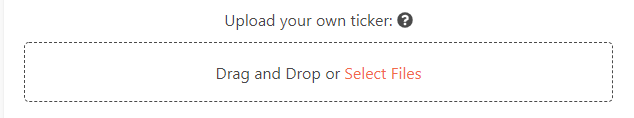
\includegraphics[scale=0.8]{08Appendices/081User/081Pictures/user_csv_alt.png}
   \caption{User Uploaded Data Field}
\end{figure}

\subsection{Viewing the Results}

The results of the backtesting process are divided between the remaining tabs of the dashboard. Let us now discuss what each of them tells the user

\subsubsection{Summary}

If all required fields are populated, the user is taken to the `Summary` tab. This, as well as all other tabs, are now unlocked. At this point, the user is shown one of the key components of our application, i.e. the portfolio growth graph. All graphs are fully interactive. The user may zoom in on selected areas, hover over desired data points, save the plot as an image, etc. The graphs can be reset by double clicking on them.

\begin{figure}[H]
   \centering
   
\includegraphics[width=\textwidth]{08Appendices/081User/081Pictures/dash_funcionalities.png}
   \caption{Dash Functionalities}
   \label{dash_functionalities}
\end{figure}

The plot seen at the top of \figurename{\ref{summary}} shows the total return of each portfolio. Users will typically use this graph for comparison. In addition, for each portfolio the user has specified, the following is shown:

\begin{itemize}
    \item Selected Key Metrics: Final Balance, Best Year, Worst Year, etc.
    \item Pie Chart: Proportion of each asset.
    \item Bar Chart: Shows how the total return changed over the years relative to the last.
\end{itemize}

\begin{figure}[H]
   \centering
   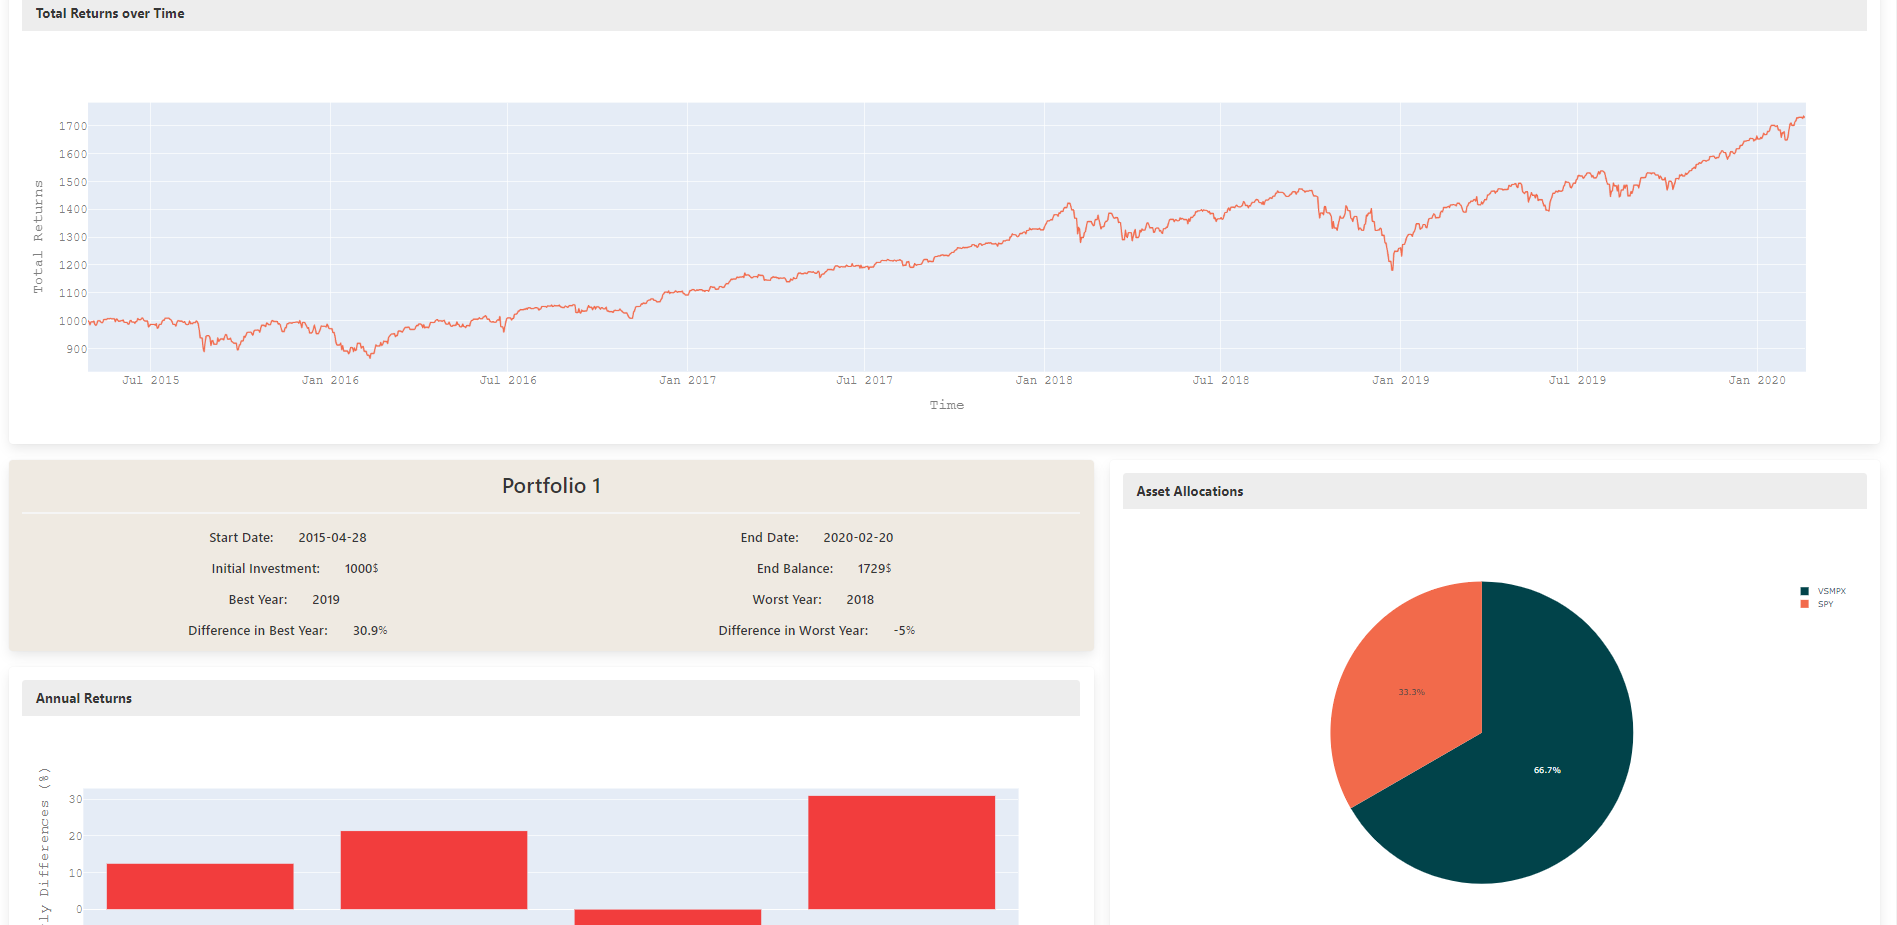
\includegraphics[width=\textwidth]{08Appendices/081User/081Pictures/summary.png}
   \caption{Summary Tab (source: http://thaliabacktest.xyz/dashboard/)}
   \label{summary}
\end{figure}

It is also important to note that in some cases, there is no data for a given asset. For example, there is no price data for cryptocurrencies before the 2000s as they did not yet exist. In edge cases where the portfolio is made up entirely of such assets, the strategy may not be valid over a given investment period. 
%It wouldn't, but what does the user see when the

If there is only one portfolio given as input, and it is affected by the above, the simulation will be run over the largest possible time frame over which data for all assets is available. In the case where the user provides multiple portfolios with different time frames, we provide output where price data is available.

\begin{figure}[H]
   \centering
   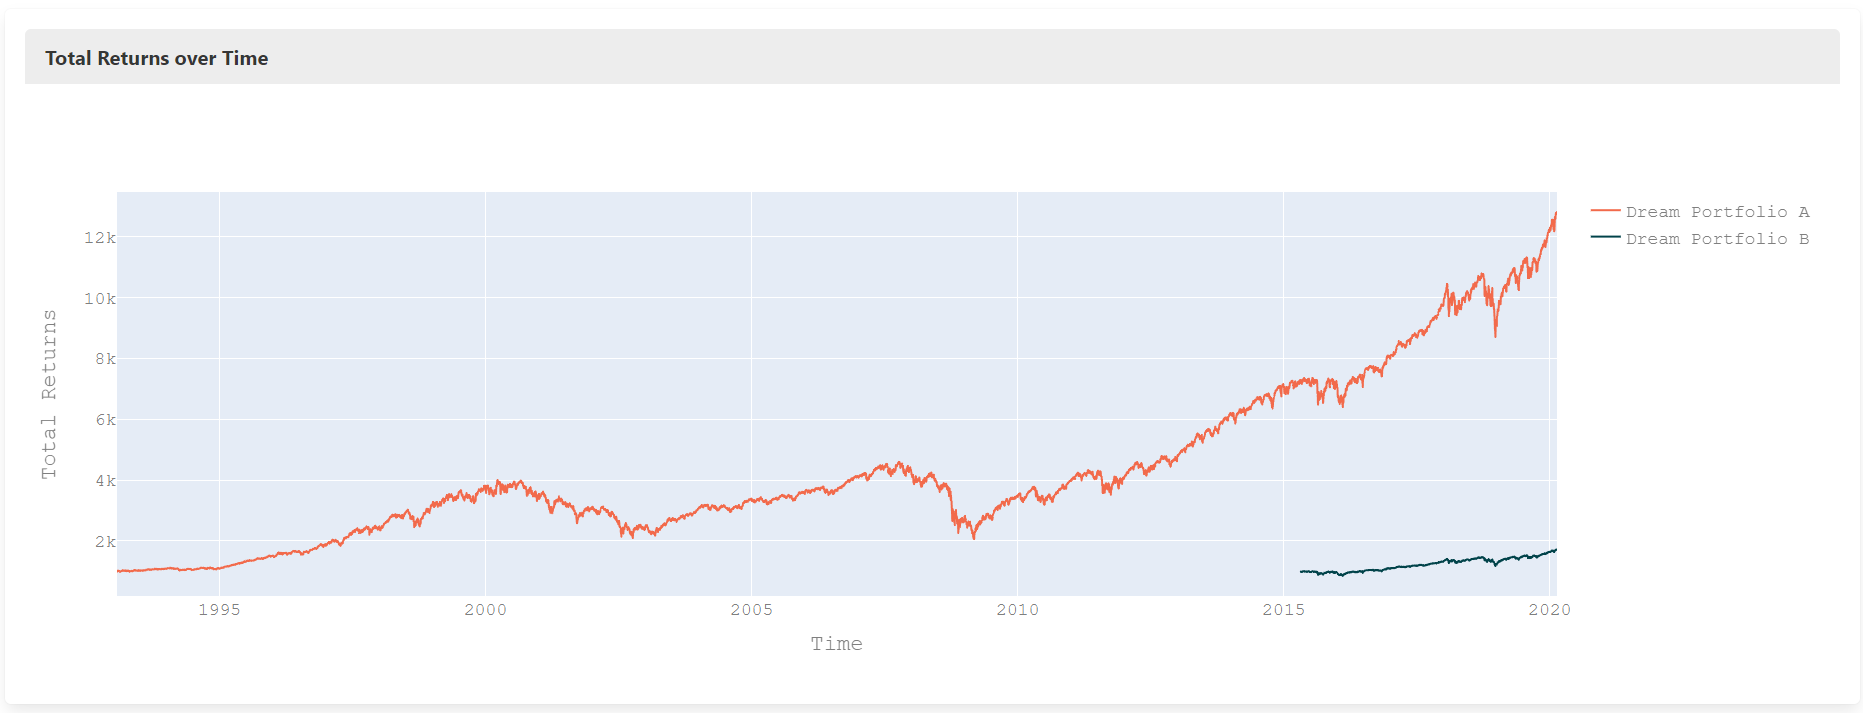
\includegraphics[width=\textwidth]{08Appendices/081User/081Pictures/differences.png}
   \caption{Different Time Frames per Portfolio (source: http://thaliabacktest.xyz/dashboard/)}
\end{figure}

\subsubsection{Metrics}

The `Metrics` tab shows a simple table of key metrics for each portfolio. This allows for a quick comparison of strategies. Although this page does not show much more data than the previous one, it can easily be expanded later. In case the table is bigger than the browser window, the user can also easily scroll down to see the rest of the output.


\begin{figure}[H]
   \centering
   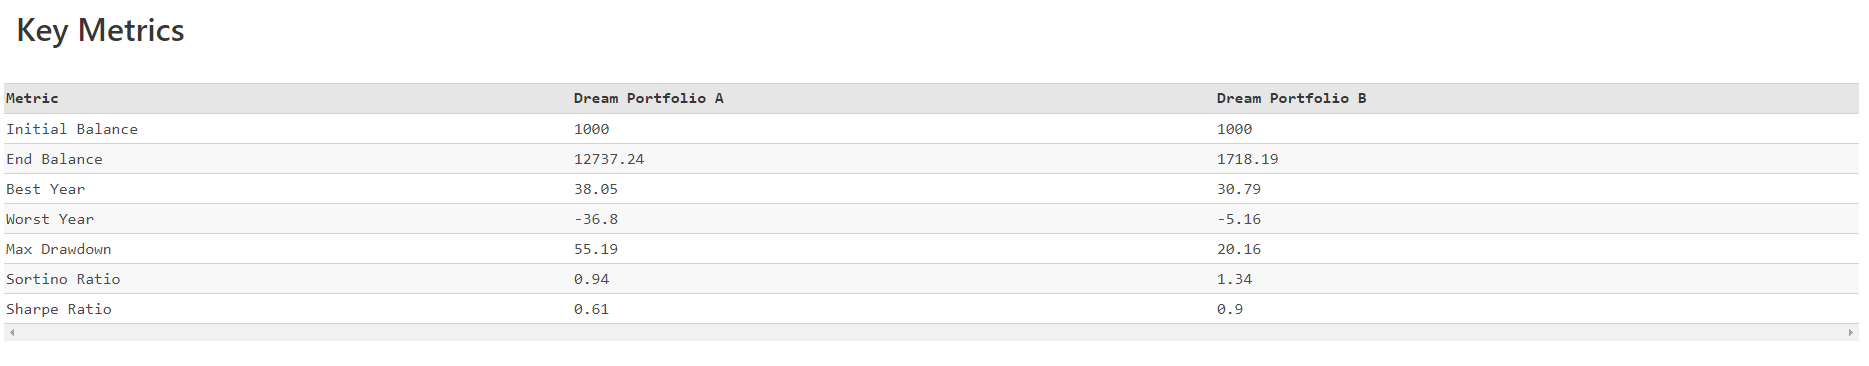
\includegraphics[width=\textwidth]{08Appendices/081User/081Pictures/metrics.png}
   \caption{Metrics Tab (source: http://thaliabacktest.xyz/dashboard/)}
   \label{metrics}
\end{figure}


\subsubsection{Returns}

The `Returns` tab allows the user to compare the annual returns of each portfolio. It consists of a bar chart similar to the one in the Summary tab and a table similar to the one in the Metrics tab. The graph can be seen on \figurename{\ref{returns}}.

\begin{figure}[H]
   \centering
   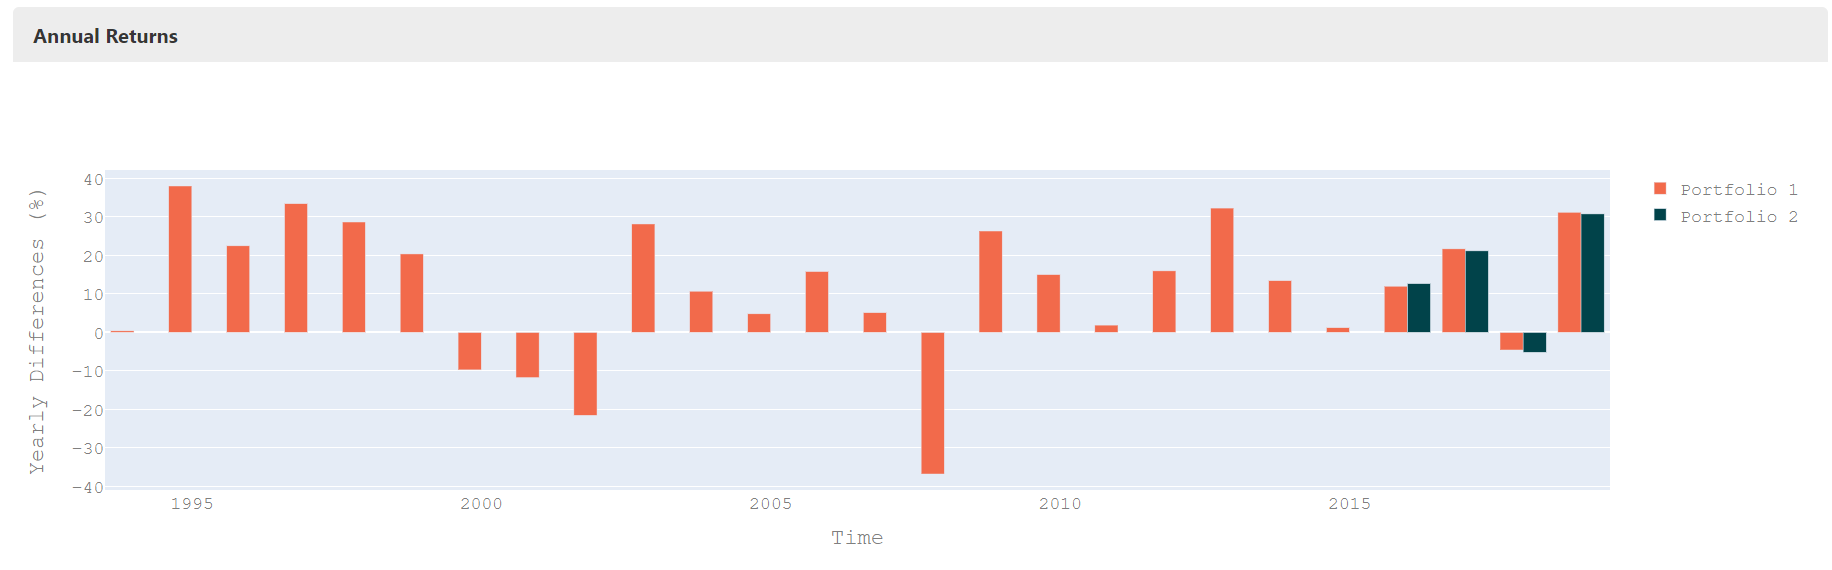
\includegraphics[width=\textwidth]{08Appendices/081User/081Pictures/returns_graph.png}
   \caption{Metrics Tab (source: http://thaliabacktest.xyz/dashboard/)}
   \label{returns}
\end{figure}

It may happen that one of the portfolios is not available at certain times as there is no data for its assets. In this case, no values are shown.

\subsubsection{Drawdowns}

The `Drawdowns` tab shows declines during the investment period. This is shown on a graph comparing each portfolio visible on \figurename{\ref{drawdowns_graph}}.

\begin{figure}[H]
   \centering
   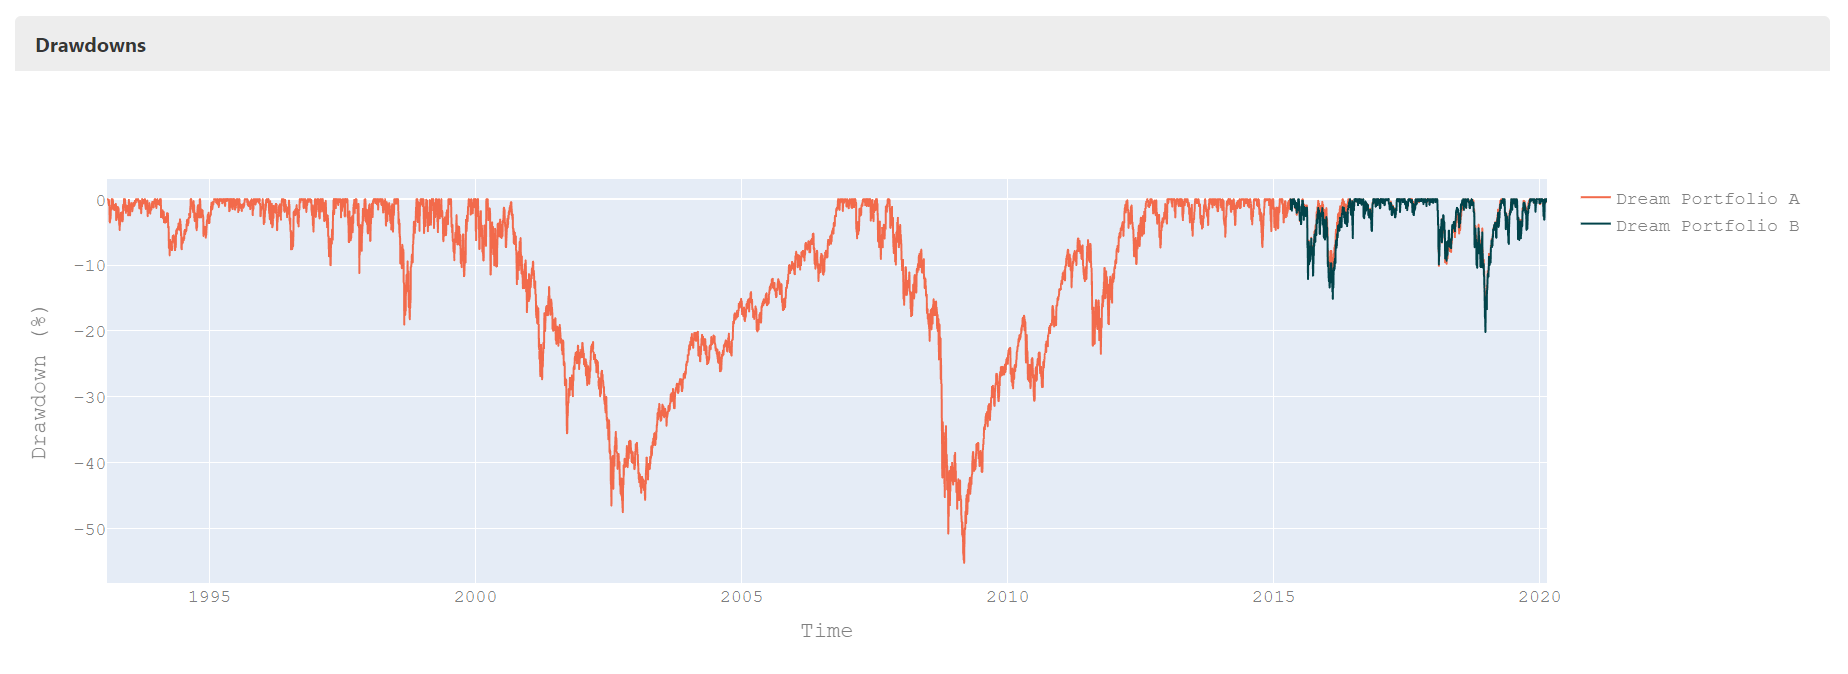
\includegraphics[width=\textwidth]{08Appendices/081User/081Pictures/drawdowns_graph.png}
   \caption{Drawdowns Tab - Graph (source: http://thaliabacktest.xyz/dashboard/)}
   \label{drawdowns_graph}
\end{figure}

For deeper insight, a table of the longest drawdowns is generated for each portfolio. By default, this will be the top 10 or as many as exist in case the portfolio does not have 10 drawdown periods.

\begin{figure}[H]
   \centering
   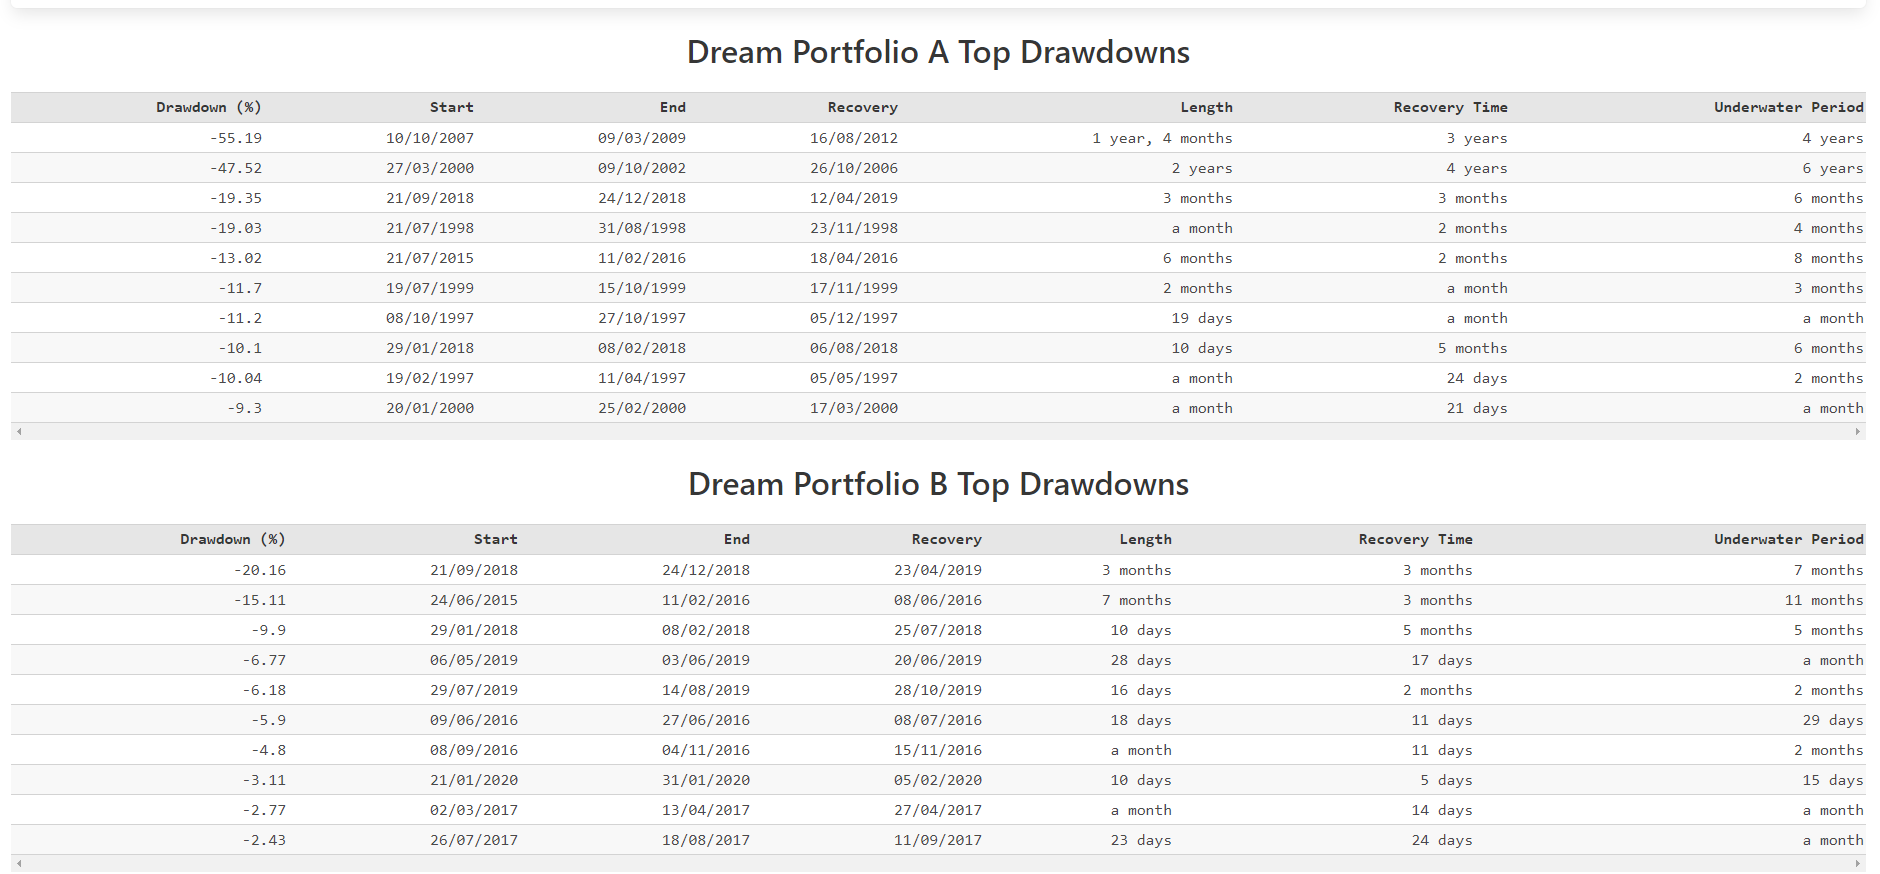
\includegraphics[width=\textwidth]{08Appendices/081User/081Pictures/drawdowns_tables.png}
   \caption{Drawdowns Tab - Tables (source: http://thaliabacktest.xyz/dashboard/)}
   \label{drawdowns_table}
\end{figure}



\subsubsection{Assets}

Here, the user may encounter a pie chart similar to the one on the summary tab. However, the pie chart shows the proportions of the asset classes as opposed to the specific assets allocated. This is crucial information for the user as it can show how diverse their portfolio truly is.

\begin{figure}[H]
   \centering
   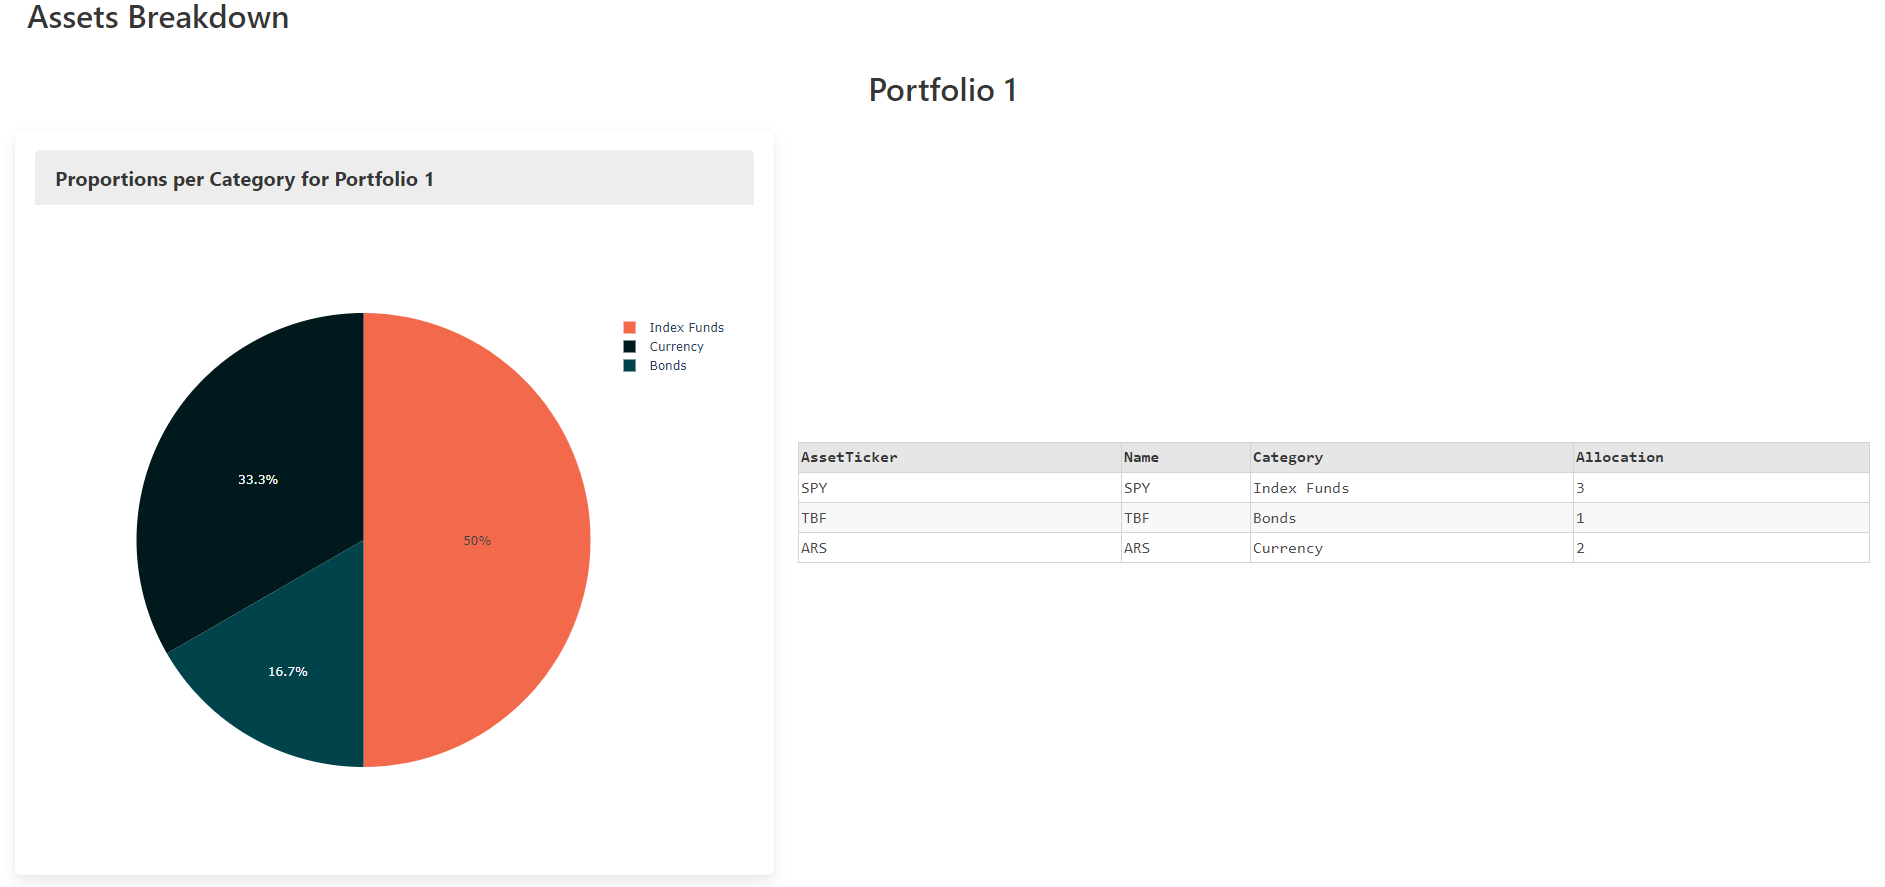
\includegraphics[width=\textwidth]{08Appendices/081User/081Pictures/assets.png}
   \caption{Assets Tab (source: http://thaliabacktest.xyz/dashboard/)}
   \label{assets_tab}
\end{figure}

\subsubsection{Overfitting}

Our last results tab encompasses a relatively complex feature, testing for overfitting. Here, the user may test if any of their portfolios exhibits bias to particular market conditions, for example by choosing a specific timeframe on witch one or more assets performs significantly better than usual (For example a simulation showing the prices of Microsoft stocks in the 90s would hardly indicate the viability of such a portfolio nowdays). Overfitting is dangerous as it may skew the investor's perception of the risk-reward characteristics of a portfolio. By clicking the button the user may opt to run an overfitting test. If it fails to detect a tendency towards overfitting in any of the selected portfolios, the following message is displayed:

\begin{figure}[H]
   \centering
   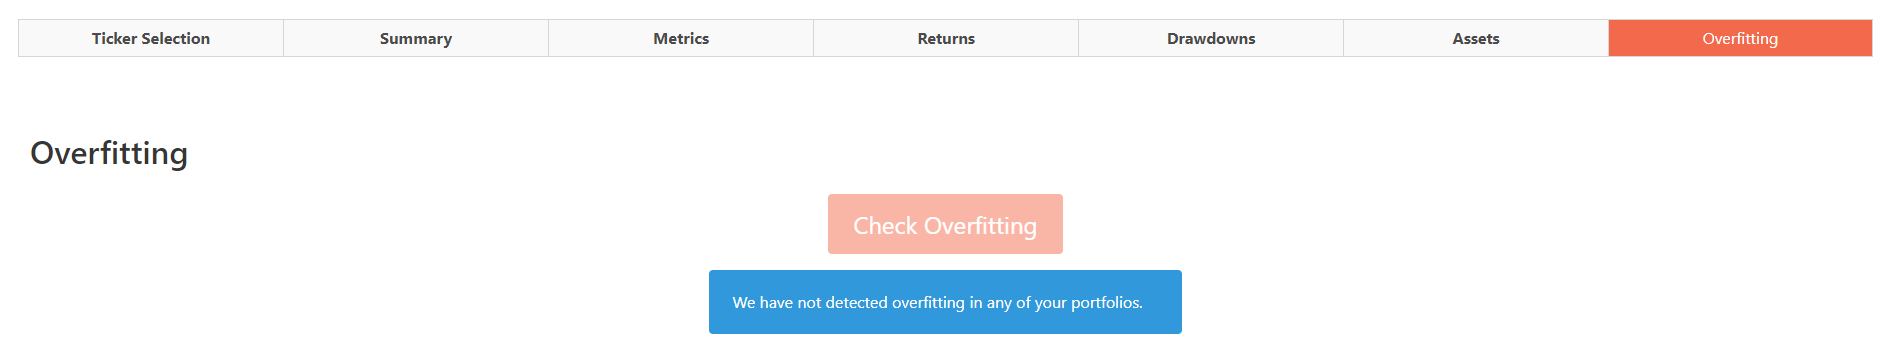
\includegraphics[width=\textwidth]{08Appendices/081User/081Pictures/overfitting.png}
   \caption{Overfitting Tab (source: http://thaliabacktest.xyz/dashboard/)}
   \label{overfitting}
\end{figure}

Alternatively, if overfitting is detected, it will warn the user, highlighting the corresponding portfolio(s).

\end{document}
